
\documentclass[]{article}

\usepackage{graphicx}
\usepackage[margin=1.5cm,top=1.5cm,bottom=1.5cm,a4paper]{geometry}
\usepackage{graphicx} % Required for inserting images
\usepackage{titlesec} % Required for customizing section titles
\usepackage[margin=1.5cm,top=1.5cm, bottom=1.5cm]{geometry} % Ajusta los márgenes aquí
\usepackage{multicol} % Required for multicols environment
\usepackage{parskip}
\usepackage{etoolbox}
\usepackage{tcolorbox}
\usepackage{float}
\usepackage{amsmath}
\usepackage{dingbat}
\usepackage{booktabs} 
\usepackage{caption}
\usepackage[utf8]{inputenc}
\usepackage[T1]{fontenc}
\usepackage{amssymb}
\usepackage[spanish]{babel}
\usepackage{multirow}
\usepackage{siunitx}
\usepackage{circuitikz}
\usepackage{pdflscape}
\usepackage{subcaption}
\usepackage{array}
\usepackage{tcolorbox}
\usepackage{xcolor}
\usepackage{pdfpages}
\usepackage{placeins}

\newif\ifcheckpoint
\checkpointfalse

% función que devuelve color según checkpoint
\newcommand{\checkpointcolor}[1]{%
	\ifcase#1
	yellow%
	\or blue%
	\or green%
	\or red%
	\or orange%
	\else gray%
	\fi
}
\newcommand{\checkpointstart}[1]{%
	\ifcheckpoint
	\edef\tempcolor{\checkpointcolor{#1}}%
	\begin{tcolorbox}[
		colback=\tempcolor!15,
		colframe=\tempcolor!60!black,
		boxrule=0pt,
		arc=0pt,
		width=\textwidth
		]
		\textbf{Inicio checkpoint #1}
	\end{tcolorbox}
	\fi
}

\newcommand{\checkpointend}[1]{%
	\ifcheckpoint
	\edef\tempcolor{\checkpointcolor{#1}}%
	\begin{tcolorbox}[
		colback=\tempcolor!15,
		colframe=\tempcolor!60!black,
		boxrule=0pt,
		arc=0pt,
		width=\textwidth
		]
		\textbf{Fin checkpoint #1}
	\end{tcolorbox}
	\fi
}

\usepackage{tikz}
\usetikzlibrary{arrows.meta, positioning}
\usetikzlibrary{babel}

\usepackage{csquotes}

\usepackage[
backend=biber,
style=apa,
citestyle=apa
]{biblatex}

\addbibresource{referencias.bib}


\begin{document}
	
	\begin{titlepage}
		
		\centering
		{
\includegraphics[scale=0.5]{img/Caratula.jpg}}
		
		\centerline
		
		{\bfseries\LARGE Taller de Diseño de Circuitos Electrónicos   \par}
		
		{\bfseries\LARGE TA138  \par}
		\vspace{.5cm}
		{\scshape\Large Facultad de Ingenier\'ia Universidad de Buenos Aires \par}
		\vspace{1.5cm}
		%{\scshape\Huge Trabajo Pr\'actico \par}
		{\scshape\Huge Diseño de Fuente de Alimentación \par}
		\vspace{2cm}
		{\scshape\Large Checkpoint 3: Caracterización y validación de regulador lineal con lazo de tensión y corriente.\par}
		
		
		\vspace{2cm}
		
		\begin{tabular}{ p{4cm} p{2cm} p{4cm}}
			\textbf{Alumnos:} & \textbf{Padr\'on:} & \textbf{Mail:} \\
			Lazo, Sebastian Nahuel & 106213 &slazo@fi.uba.ar \\
			Flores, Ahmed Ali & 106238 & aaflores@fi.uba.ar  \\
			Mántaras, Ramiro  & 111510 &rmantaras@fi.uba.ar \\
			
		\end{tabular}
		
		
		\vspace{1cm}
		
		\begin{tabular}{ p{6cm} p{6cm} p{6cm}}
			\textbf{Docentes:}  
			\\Teóricas: Julio Zola & Tutor: Sergio Andres Quinteros  
		\end{tabular}
		
	\end{titlepage}
	
	
	\newpage
	
	
	\tableofcontents \label{Indice}
	\newpage
	
	\checkpointstart{1}
	\section{Objetivo}

	Continuando con el diseño de un regulador lineal que cumpla con las especificaciones definidas en informes previos, en este \textit{checkpoint} se avanza hacia su implementación en un prototipo de circuito impreso (PCB), con el fin de caracterizar y validar experimentalmente las prestaciones obtenidas en la etapa de diseño.
	
	\section{Desarrollo}
	
	Para el desarrollo de este \textit{checkpoint 3} se adquirieron los materiales siguiendo el listado de partes y proveedores detallada en el apéndice \ref{sec:apendice_presupuesto}.
	

	
	\subsection{Fabricación de la PCB}
	
	Tomando como referencia el diseño del circuito impreso presentado en el \textit{checkpoint 2} al que se le realizaron correcciones llegando finalmente al diseño fabricado, el cual se puede apreciar en el apéndice \ref{sec:apendice_PCB}, luego se dio paso a el proceso de fabricación del prototipo del PCB.
	
	Se utilizo el método de "planchado" a una placa de cobre FR4 marcando las pistas por medio de papel impreso de transferencia térmica aplicándole calor. Luego se sumergió la placa en cloruro férrico atacando el cobre sobrante.
		
	Luego, se aplicó la serigrafía superior utilizando el mismo método (véase Figura~\ref{fig:placamontada1}). A continuación, se realizaron las perforaciones correspondientes, se limpió la placa con alcohol isopropílico y se procedió al ensamblado del circuito mediante la colocación de los componentes y soldado adecuado.
	
	\begin{figure}[H]
		\centering
		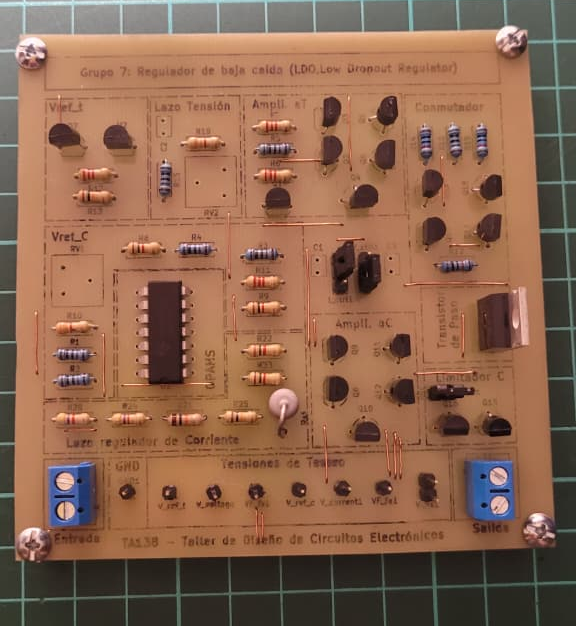
\includegraphics[width=0.8\linewidth]{img/LDO/Placa_montada_1}
		\caption{Placa montada.}
		\label{fig:placamontada1}
	\end{figure}

	

	\subsection{Mediciones}
	  
	  Con el objetivo de validar experimentalmente el desempeño del regulador implementado, se llevaron a cabo una serie de mediciones sobre el prototipo construido. Estas pruebas permiten contrastar los resultados obtenidos en la etapa de diseño y simulación con el comportamiento real del circuito, evaluando parámetros clave como la regulación de carga, la regulación de línea, la capacidad de limitación de corriente y la eficiencia del sistema. A continuación, se describe el banco de pruebas utilizado y la metodología empleada en cada caso.
	
	\subsubsection{Banco de Pruebas}
	
	Para realizar las mediciones se llevo la placa a el laboratorio y se la dispuso frente a un banco de pruebas compuesto por los siguientes instrumentos de medición.
	
	%completar al medir
	\begin{itemize}
		\item Fuente : UNI-T, UTP33115TFL-II
		\item Generador
		\item Osciloscopio : UNI-T, UTD2102CEX+
		\item Multimetro: VT-POWER, M890G
	\end{itemize}

	\begin{figure}[H]
		\centering
		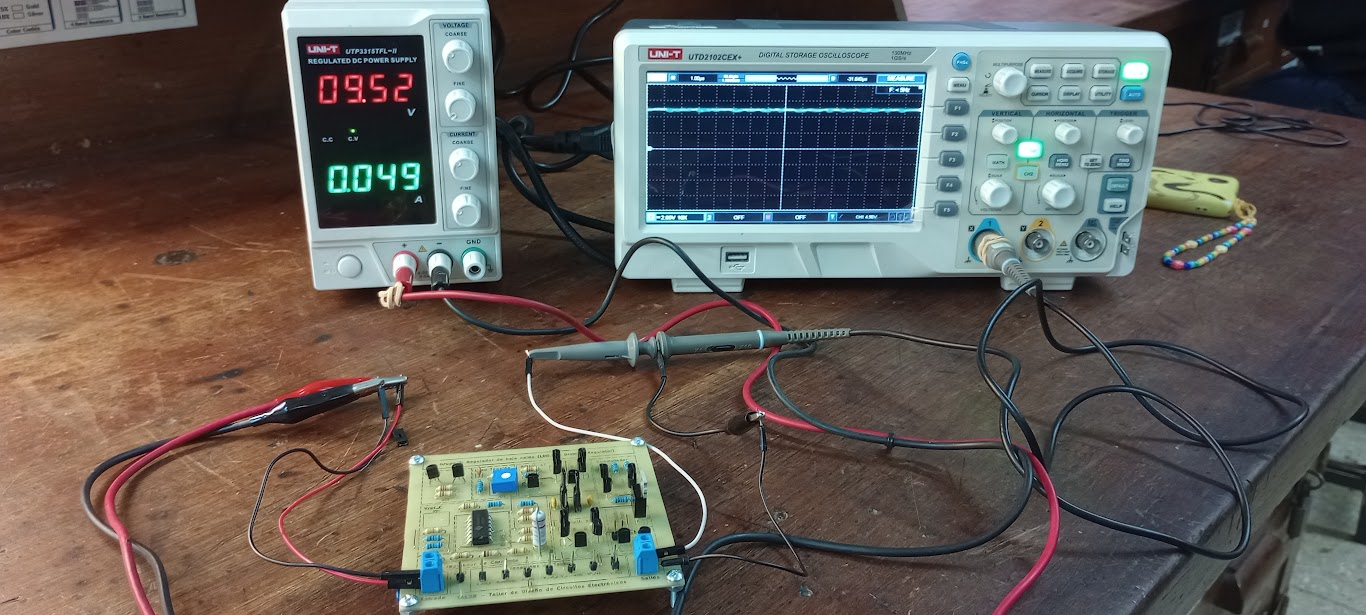
\includegraphics[width=1\linewidth]{img/LDO/banco_medicion}
		\caption{banco de medición en laboratorio.}
		\label{fig:bancomedicion}
	\end{figure}
	

	\subsubsection{Análisis de confiabilidad de los componentes}
	
	Se debe tener en cuenta que los fabricantes disponen de un rango para los parámetros característicos de cada componente, los cuales pueden variar de acuerdo a sus condiciones ambientales, de funcionamiento y de fabricación, pudiendo un lote variar respecto a otro y, a su vez, cada componente individualmente.
	
	En este sentido, el análisis de confiabilidad del circuito requiere contemplar dichas dispersiones mediante técnicas de verificación y modelización que permitan estimar su impacto en el desempeño global. Una de las metodologías empleadas consiste en la evaluación de condiciones de peor caso (worst-case), considerando los valores extremos especificados en las hojas de datos para parámetros críticos como ganancia en corriente ($\beta$) en transistores bipolares, tensión umbral en MOSFETs, tensión de referencia en dispositivos como el TL431, offset y ganancia en lazo abierto en amplificadores operacionales, y tolerancias en resistencias.
	
	
	Se realizaron mediciones del parámetro de ganancia de corriente continua \(h_{FE}\) en doce transistores BC547 utilizando un multímetro VT-POWER M890G. Los valores obtenidos fueron:
	
	\[
	328,\ 342,\ 325,\ 337,\ 332,\ 322,\ 334,\ 328,\ 320,\ 320,\ 318,\ 318
	\]
	
	El valor promedio medido resulta:
	
	\[
	\overline{\beta}=
	\frac{1}{12}\sum_{i=1}^{12}\beta_i
	\approx 327
	\]
	
	Asimismo, se obtuvo una desviación estándar aproximada de:
	
	\[
	\sigma \approx 7.7
	\]
	
	Los valores medidos se encuentran dentro del siguiente rango experimental:
	
	\[
	318 \leq \beta \leq 342
	\]
	
	La dispersión observada es reducida, con variaciones menores al \(5\%\) respecto del valor medio. Esto indica una buena uniformidad paramétrica entre los dispositivos analizados, permitiendo estimar un valor típico de diseño de:
	
	\[
	\beta \approx 330
	\]
	
	A partir de los resultados obtenidos, puede concluirse que los transistores presentan un comportamiento consistente y repetible dentro del lote analizado, resultando adecuados para aplicaciones analógicas de pequeña señal donde la estabilidad de ganancia y la confiabilidad de los componentes son relevantes.
	
	
	\begin{table}[H]
		\centering
		\caption{Comparación de parámetros teóricos y medidos experimentalmente}
		\label{tab:comparacion_componentes}
		\begin{tabular}{|c|c|c|c|}
			\hline
			\textbf{Componente} & \textbf{Parámetro} & \textbf{Valor teórico} & \textbf{Valor medido} \\
			\hline
			
			\multirow{2}{*}{TL431} 
			& $V_{ref}$ (V) & 2.495 & 2,45 \\
			& $I_{ref}$ (µA) & 2 -- 4 & --- \\
			\hline
			
			\multirow{3}{*}{LM324} 
			& $V_{os}$ (mV) & 2 (típ.) & --- \\
			& $A_{OL}$ (dB) & 100 (típ.) & --- \\
			& $I_{bias}$ (nA) & 20 (típ.) & --- \\
			\hline
			
			\multirow{2}{*}{2N3904} 
			& $\beta$ (hFE) & 100 -- 300 & 271 \\
			& $V_{BE}$ (V) & 0.65 -- 0.7 & 0,66 \\
			\hline
			
			\multirow{2}{*}{2N3906} 
			& $\beta$ (hFE) & 100 -- 300 & 273 \\
			& $V_{BE}$ (V) & 0.65 -- 0.7 & 0,67 \\
			\hline
			
			\multirow{2}{*}{BC547} 
			& $\beta$ (hFE) & 300 -- 500 & 330 \\
			& $V_{BE}$ (V) & 0.65 -- 0.7 & 0,67 \\
			\hline
			
			\multirow{2}{*}{BC557} 
			& $\beta$ (hFE) & 300 -- 500 & 304 \\
			& $V_{BE}$ (V) & 0.65 -- 0.7 & 0,67 \\
			\hline
			
		\end{tabular}
	\end{table}
	%Completar luego de medir
	Con los resultados obtenidos se puede esperar un desvío en los resultados hacia... 
	
	\subsubsection{Regulación de carga estática y dinámica}
	
	\subsubsection{Regulación de línea}
	
	\subsubsection{Limitación de corriente}
	
	\subsubsection{Eficiencia}


	
\section{Conclusiones}

A lo largo del desarrollo del presente trabajo se logró caracterizar experimentalmente un regulador lineal LDO discreto, evaluando su comportamiento estático y dinámico mediante distintas metodologías de medición. La comparación entre los resultados experimentales y las simulaciones realizadas en LTspice permitió validar gran parte de los modelos teóricos empleados durante el diseño, observándose una buena correlación tanto en la regulación de tensión como en la respuesta frente a variaciones de carga y alimentación. Mientras que en la limitación de corriente las mediciones permitieron verificar una discrepancia con el diseño de 500 mA, lo cual es un error critico y no deseado.

A partir de la interpolación y análisis de las mediciones experimentales se verificó el correcto funcionamiento de la etapa de regulación dentro de la región esperada, incluyendo el comportamiento del \textit{dropout}, la regulación de línea, la regulación de carga y la eficiencia del sistema. Asimismo, los ensayos dinámicos mediante carga activa permitieron observar la respuesta transitoria del regulador frente a cambios abruptos de corriente, obteniéndose una dinámica subamortiguada coherente con la prevista en simulación, aunque con amplitudes superiores debido a efectos no ideales presentes en la implementación física.

Durante el desarrollo experimental también se identificó una discrepancia importante respecto de las simulaciones iniciales: en una primera instancia no se consideró adecuadamente el nodo correspondiente al limitador de corriente, lo cual introdujo una oscilación adicional  de aproximadamente 16 kHz no contemplada en el checkpoint previo. Este fenómeno evidenció la sensibilidad del sistema frente a polos y acoplamientos parásitos asociados a la etapa de limitación de corriente. A partir del análisis posterior se determinó que la incorporación de un capacitor de compensación de aproximadamente $100\ \text{pF}$ entre base y colector del transistor NPN del limitador permitiría estabilizar dicho nodo, reduciendo significativamente la tendencia oscilatoria observada.

En términos generales, el trabajo permitió no sólo validar experimentalmente los conceptos teóricos asociados al diseño de reguladores lineales LDO, sino también adquirir experiencia práctica en simulación analógica, compensación en frecuencia, caracterización experimental y análisis de estabilidad en sistemas electrónicos reales. La comparación entre teoría, simulación e implementación física resultó fundamental para comprender las limitaciones de los modelos ideales y la influencia de las no idealidades presentes en circuitos electrónicos discretos.

	{\footnotesize
		\printbibliography
	}
	
	
	\appendix
	\begin{landscape}
	\section{Apéndice I: Simulaciones}
	\label{sec:apendice_simulaciónes}
	
	\subsection{LDO}
	
	\begin{figure}[H]
		\centering
		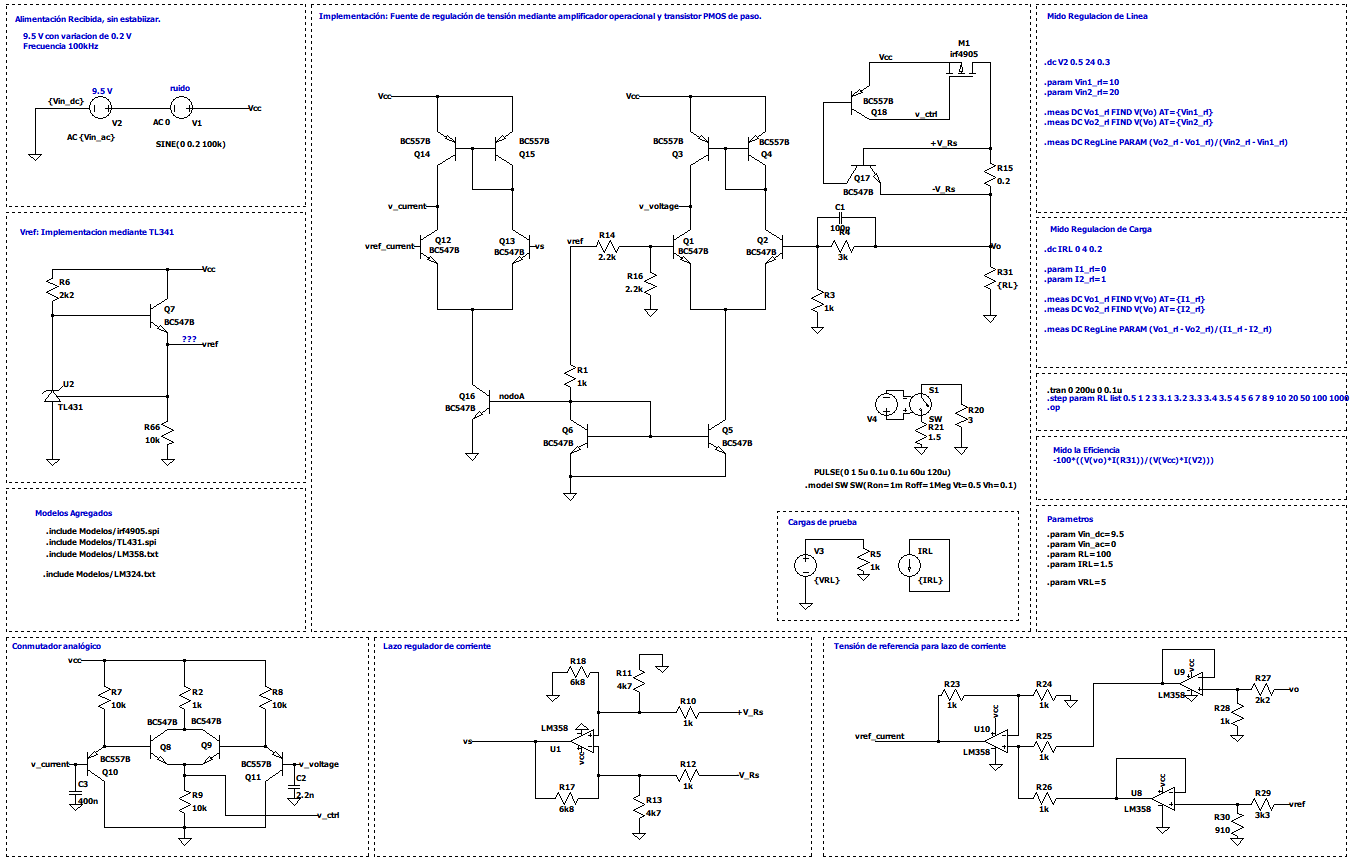
\includegraphics[width=0.85\linewidth]{img/LDO/Esquematico_LDO_LTSPICE2}
		\caption{Captura de simulación en LtSpice.}
		\label{fig:esquematicoldoltspice}
	\end{figure}

	\section{Apéndice II: Esquemáticos}
	\label{sec:apendice_esquematicos}
		
	\subsection{LDO}
	\begin{figure}[H]
		\centering
		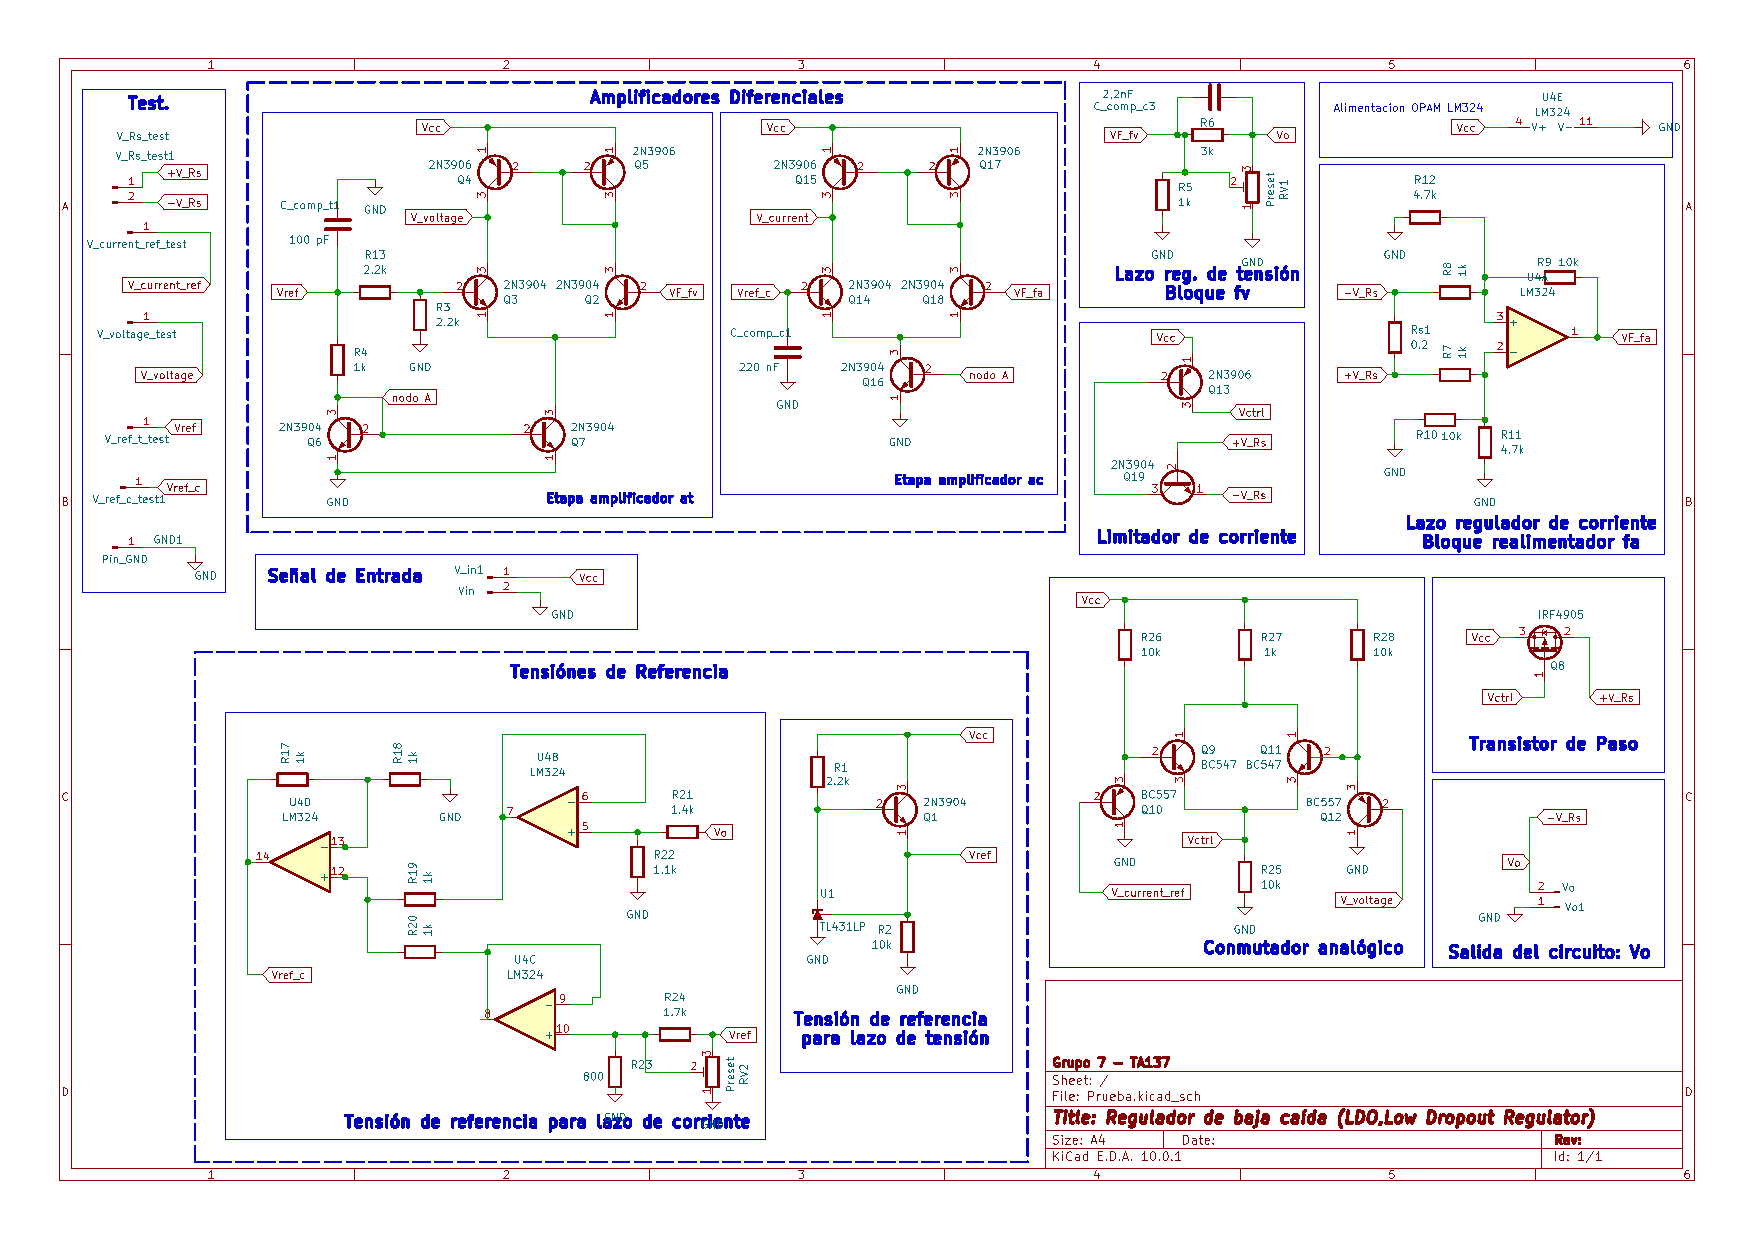
\includegraphics[width=0.85\linewidth]{img/LDO/esquematico_LDO_Kicad.pdf}
		\caption{Esquemático de la implementación del regulador lineal LDO.}
		\label{fig:esquematicokicadldo}
	\end{figure}
	\end{landscape}


\begingroup


\let\clearpage\relax

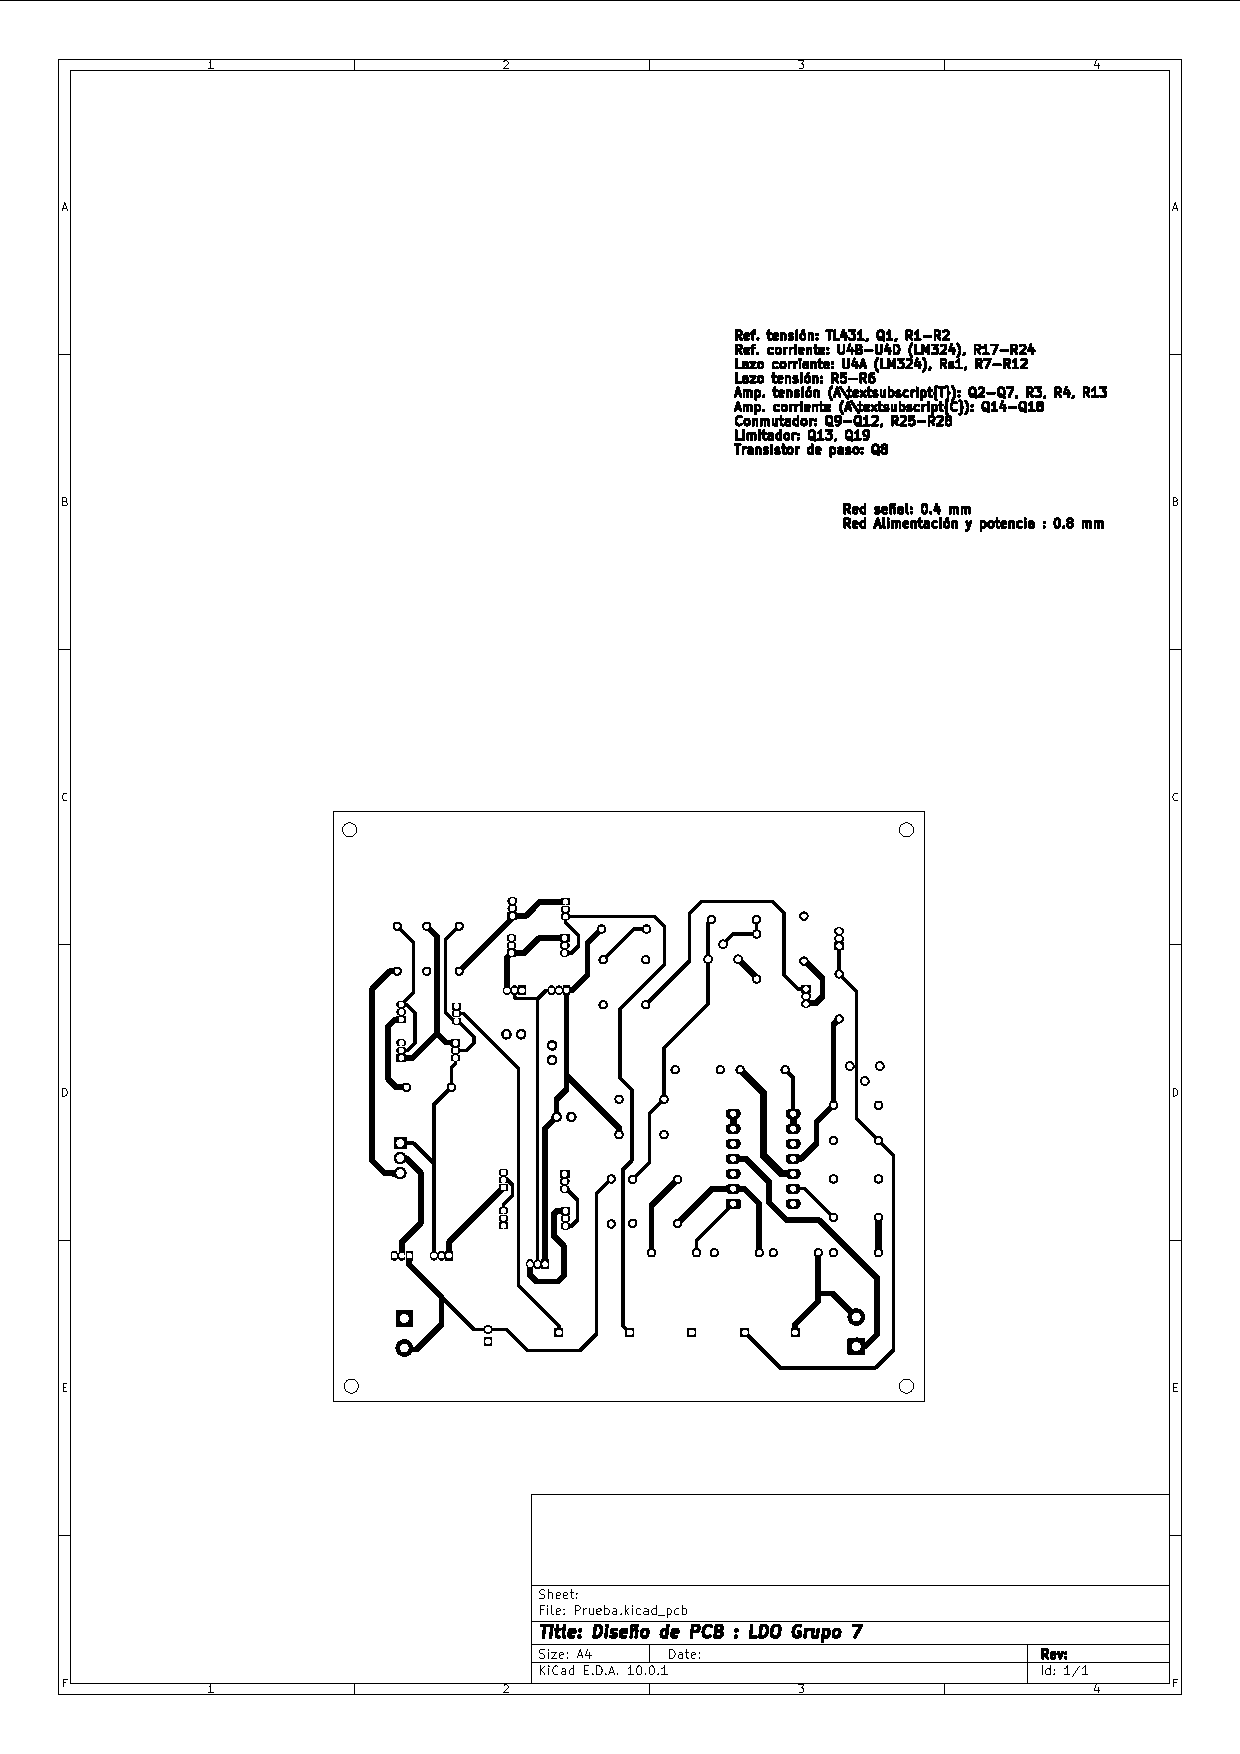
\includepdf[
pages=1,
pagecommand={\section{Apéndice III: PCB}
	\label{sec:apendice_PCB} \subsection{LDO capa superior}}
]{img/LDO/pistas_LDO.pdf}

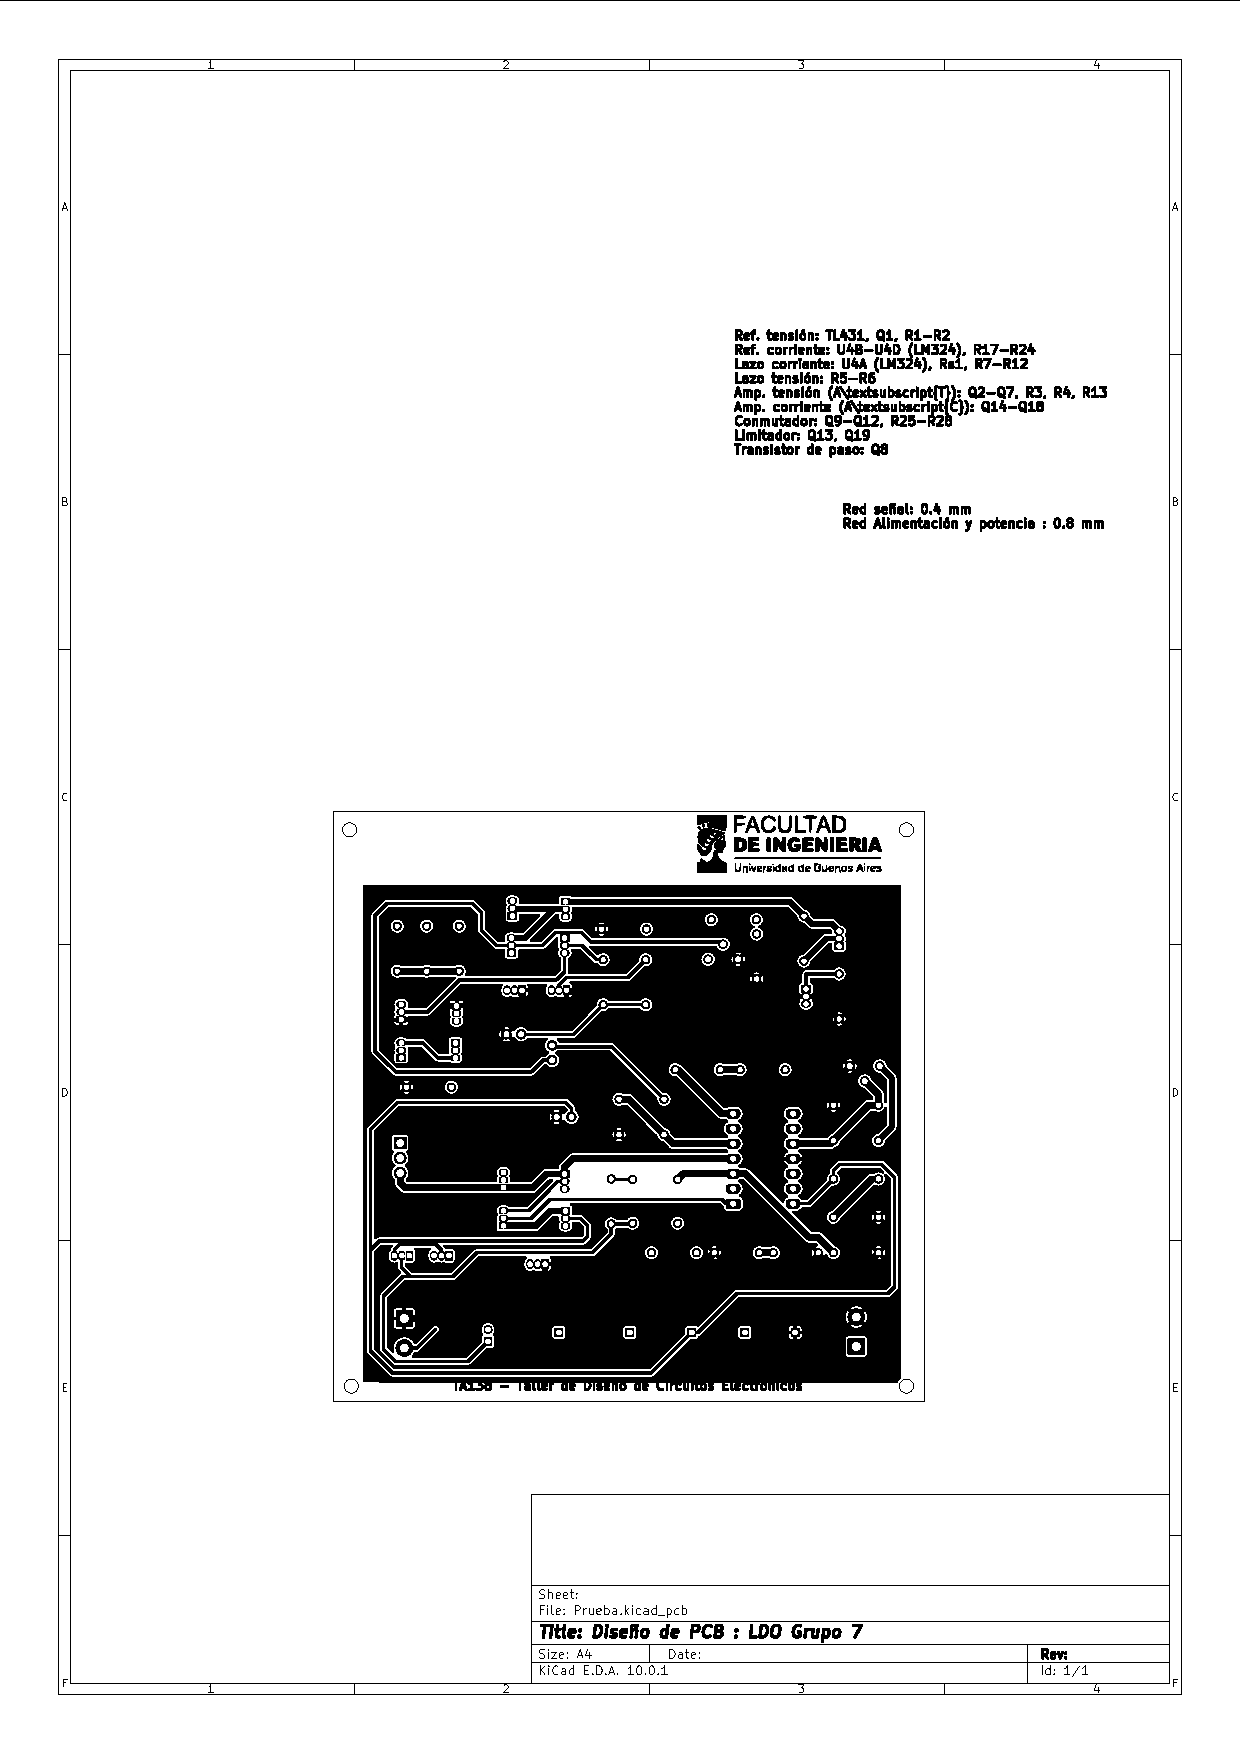
\includepdf[
pages=1,
pagecommand={\subsection{LDO capa inferior}}
]{img/LDO/pistas_LDO_inferior.pdf}

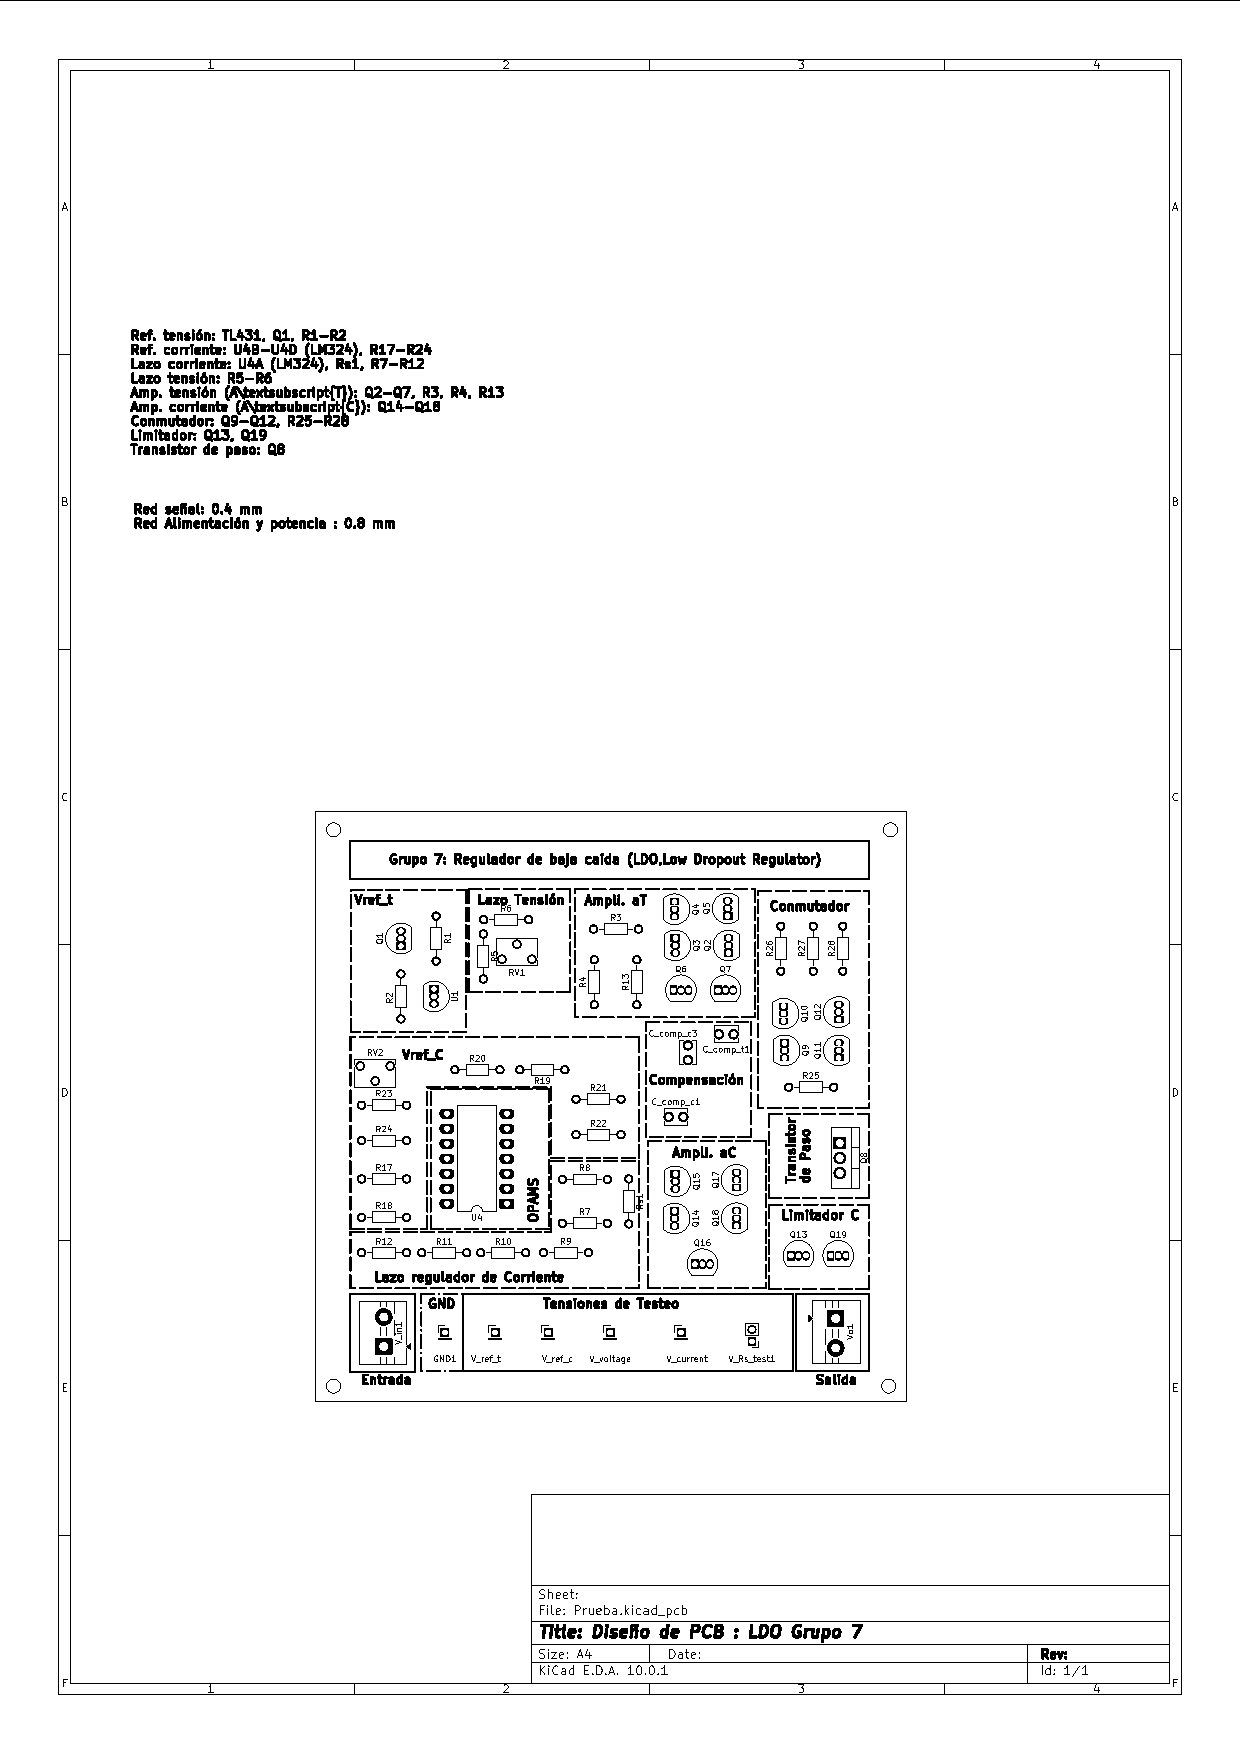
\includepdf[
pages=1,
pagecommand={\subsection{LDO Serigrafía superior}}
]{img/LDO/Serigrafia_LDO_superior.pdf}


\endgroup



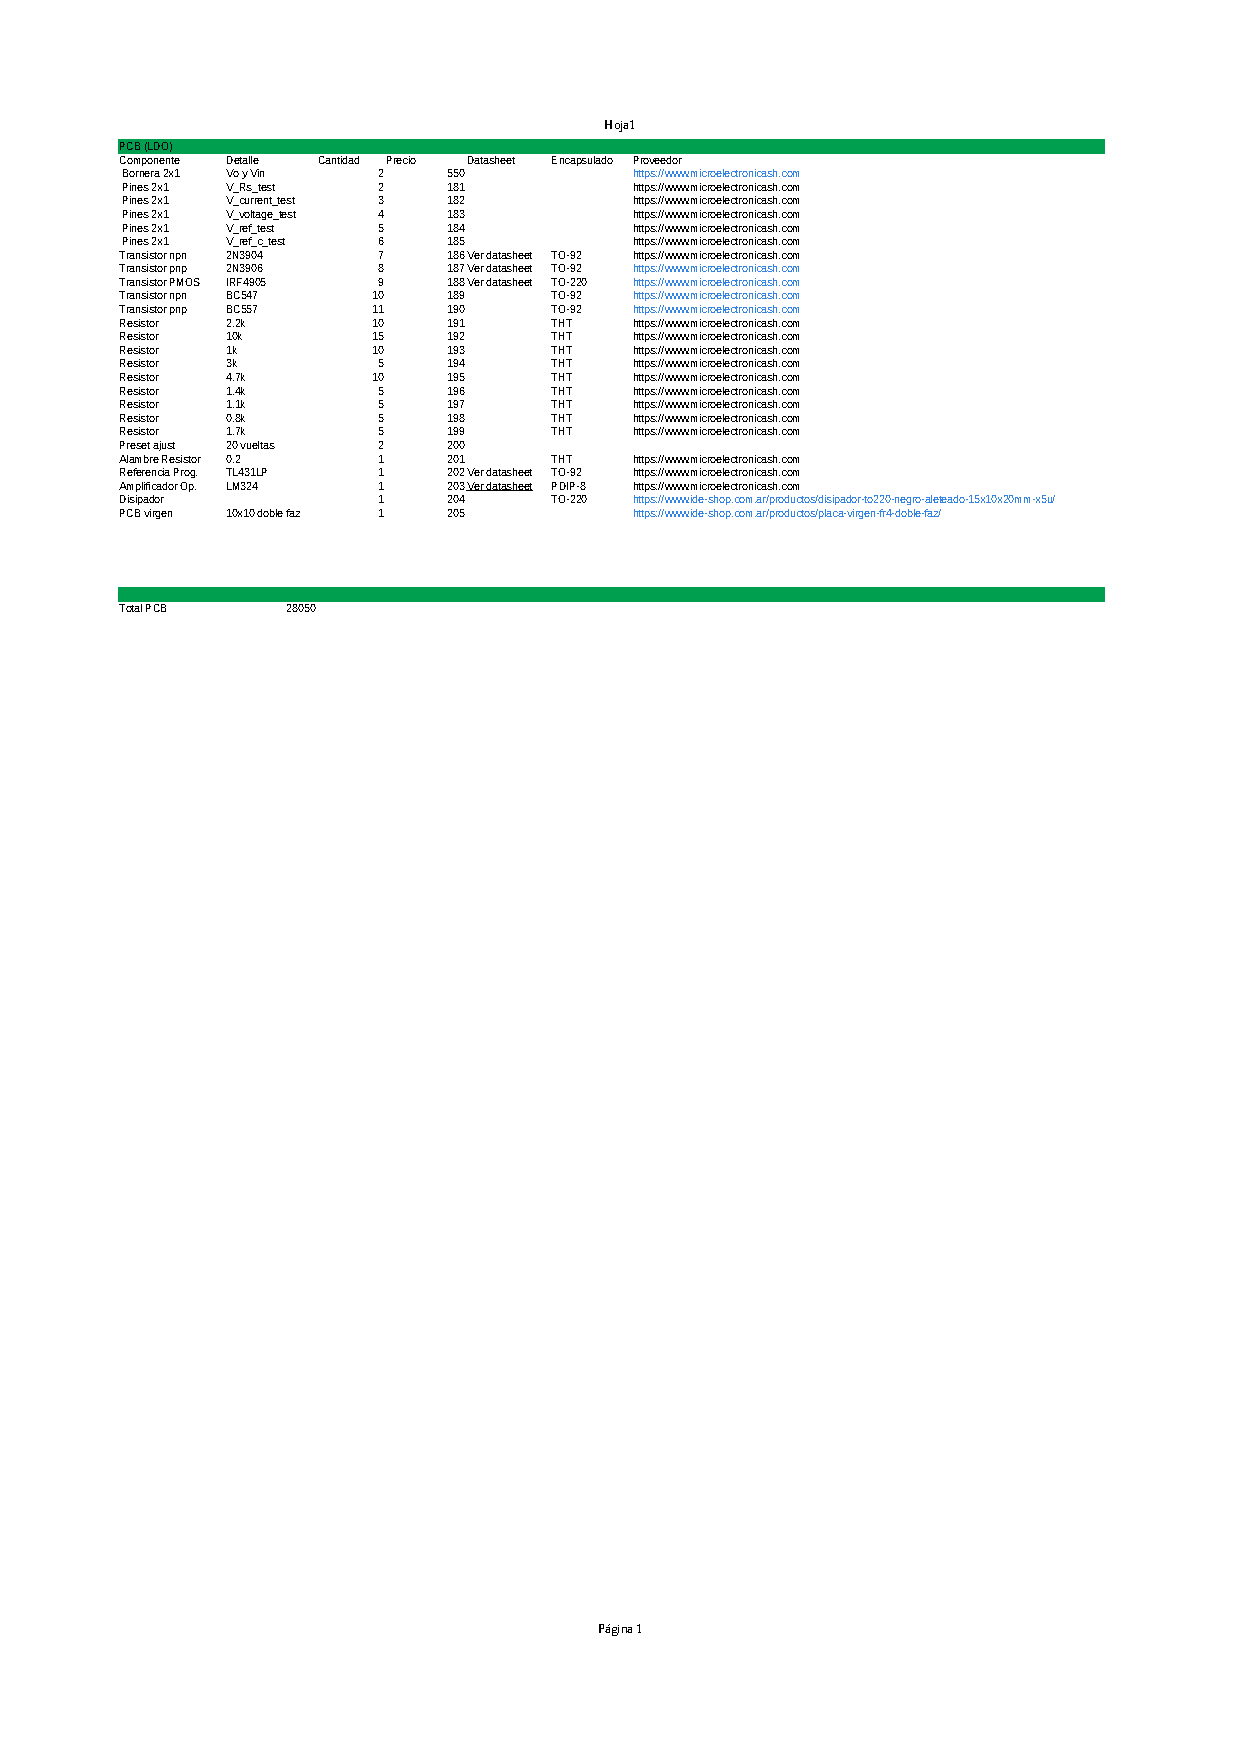
\includepdf[
pages=1,
pagecommand={\section{Apéndice IV: Presupuesto}
	\label{sec:apendice_presupuesto}
}
]{img/LDO/Presupuesto.pdf}



\end{document}
